\documentclass{article}
\usepackage{xcolor}
\newcommand{\red}{\color{red}}
\usepackage{tikz}
\usepackage[width=200mm]{geometry}
\pagestyle{empty}

\begin{document}

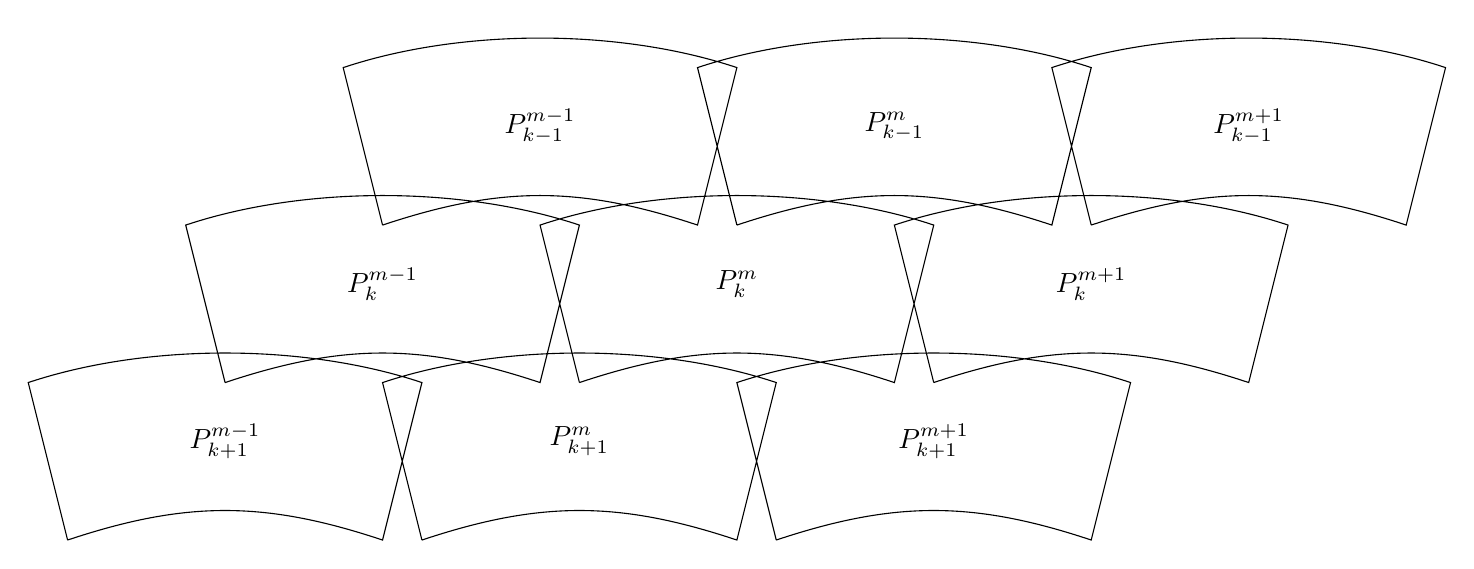
\begin{tikzpicture}
	%\draw[help lines] (-1,-1) grid (12,6);
	\draw
	%% P
	% m-1
	(-2,-2) .. controls +(1.5,.5) and +(-1.5,.5) .. ++(4,0)
	-- ++(.5,2) .. controls +(-1.5,.5) and +(1.5,.5) .. ++(-5,0)
	-- ++(.5,-2,0) +(2,1.25) node{$P_{k+1}^{m-1}$}
	(0,0) .. controls +(1.5,.5) and +(-1.5,.5) .. ++(4,0)
	-- ++(.5,2) .. controls +(-1.5,.5) and +(1.5,.5) .. ++(-5,0)
	-- ++(.5,-2,0) +(2,1.25) node{$P_{k}^{m-1}$}
	(2,2) .. controls +(1.5,.5) and +(-1.5,.5) .. ++(4,0)
	-- ++(.5,2) .. controls +(-1.5,.5) and +(1.5,.5) .. ++(-5,0)
	-- ++(.5,-2,0) +(2,1.25) node{$P_{k-1}^{m-1}$}
	% m
	(2.5,-2) .. controls +(1.5,.5) and +(-1.5,.5) .. ++(4,0)
	-- ++(.5,2) .. controls +(-1.5,.5) and +(1.5,.5) .. ++(-5,0)
	-- ++(.5,-2,0) +(2,1.25) node{$P_{k+1}^{m}$}
	(4.5,0) .. controls +(1.5,.5) and +(-1.5,.5) .. ++(4,0)
	-- ++(.5,2) .. controls +(-1.5,.5) and +(1.5,.5) .. ++(-5,0)
	-- ++(.5,-2,0) +(2,1.25) node{$P_{k}^{m}$}
	(6.5,2) .. controls +(1.5,.5) and +(-1.5,.5) .. ++(4,0)
	-- ++(.5,2) .. controls +(-1.5,.5) and +(1.5,.5) .. ++(-5,0)
	-- ++(.5,-2,0) +(2,1.25) node{$P_{k-1}^{m}$}
	% m+1
	(7,-2) .. controls +(1.5,.5) and +(-1.5,.5) .. ++(4,0)
	-- ++(.5,2) .. controls +(-1.5,.5) and +(1.5,.5) .. ++(-5,0)
	-- ++(.5,-2,0) +(2,1.25) node{$P_{k+1}^{m+1}$}
	(9,0) .. controls +(1.5,.5) and +(-1.5,.5) .. ++(4,0)
	-- ++(.5,2) .. controls +(-1.5,.5) and +(1.5,.5) .. ++(-5,0)
	-- ++(.5,-2,0) +(2,1.25) node{$P_{k}^{m+1}$}
	(11,2) .. controls +(1.5,.5) and +(-1.5,.5) .. ++(4,0)
	-- ++(.5,2) .. controls +(-1.5,.5) and +(1.5,.5) .. ++(-5,0)
	-- ++(.5,-2,0) +(2,1.25) node{$P_{k-1}^{m+1}$}
	%% Q
	%(.3,1.8) -- ++(0,1.4) -- ++(3.4,0) -- ++(0,-1.4) -- ++(-3.4,0) +(1.75,0.75) node{$Q_{k}^{m-1}$}
	%(3.8,0.3) -- ++(0,1.4) -- ++(3.4,0) -- ++(0,-1.4) -- ++(-3.4,0) +(1.75,0.75) node{$Q_{k-1}^{m}$}
	%(3.8,3.3) -- ++(0,1.4) -- ++(3.4,0) -- ++(0,-1.4) -- ++(-3.4,0) +(1.75,0.75) node{$Q_{k}^{m}$}
	%(7.3,1.8) -- ++(0,1.4) -- ++(3.4,0) -- ++(0,-1.4) -- ++(-3.4,0) +(1.75,0.75) node{$Q_{k+1}^{m+1}$}
	;
\end{tikzpicture}

\end{document}
